% author and copyright Pavel Seda
% modified by Truong Nhan Nguyen
% created in 1/1/2022

\documentclass[tikz, border=10pt]{standalone}

% preamble
\usepackage{tikz}
\usetikzlibrary{arrows.meta}        % library contains various arrow styles
\usepackage{xcolor}

% define style
\tikzset{
    % node style
    every node/.style = {fill=white, font=\sffamily},
    % arrow style
    >={latex[width=2mm, length=2mm]},
    % abstract base node style
    base/.style = {
        draw, rectangle, rounded corners,
        minimum height=1cm, minimum width=4cm,
        text centered, font=\sffamily
    },
    % special node styles (inherited from base style)
    activityStart/.style = {base, fill=blue!30},
    startStop/.style = {base, fill=red!30},
    activityRun/.style = {base, fill=green!30},
    process/.style = {base, fill=orange!30, minimum width=2.5cm, font=\ttfamily}
}

\begin{document}
    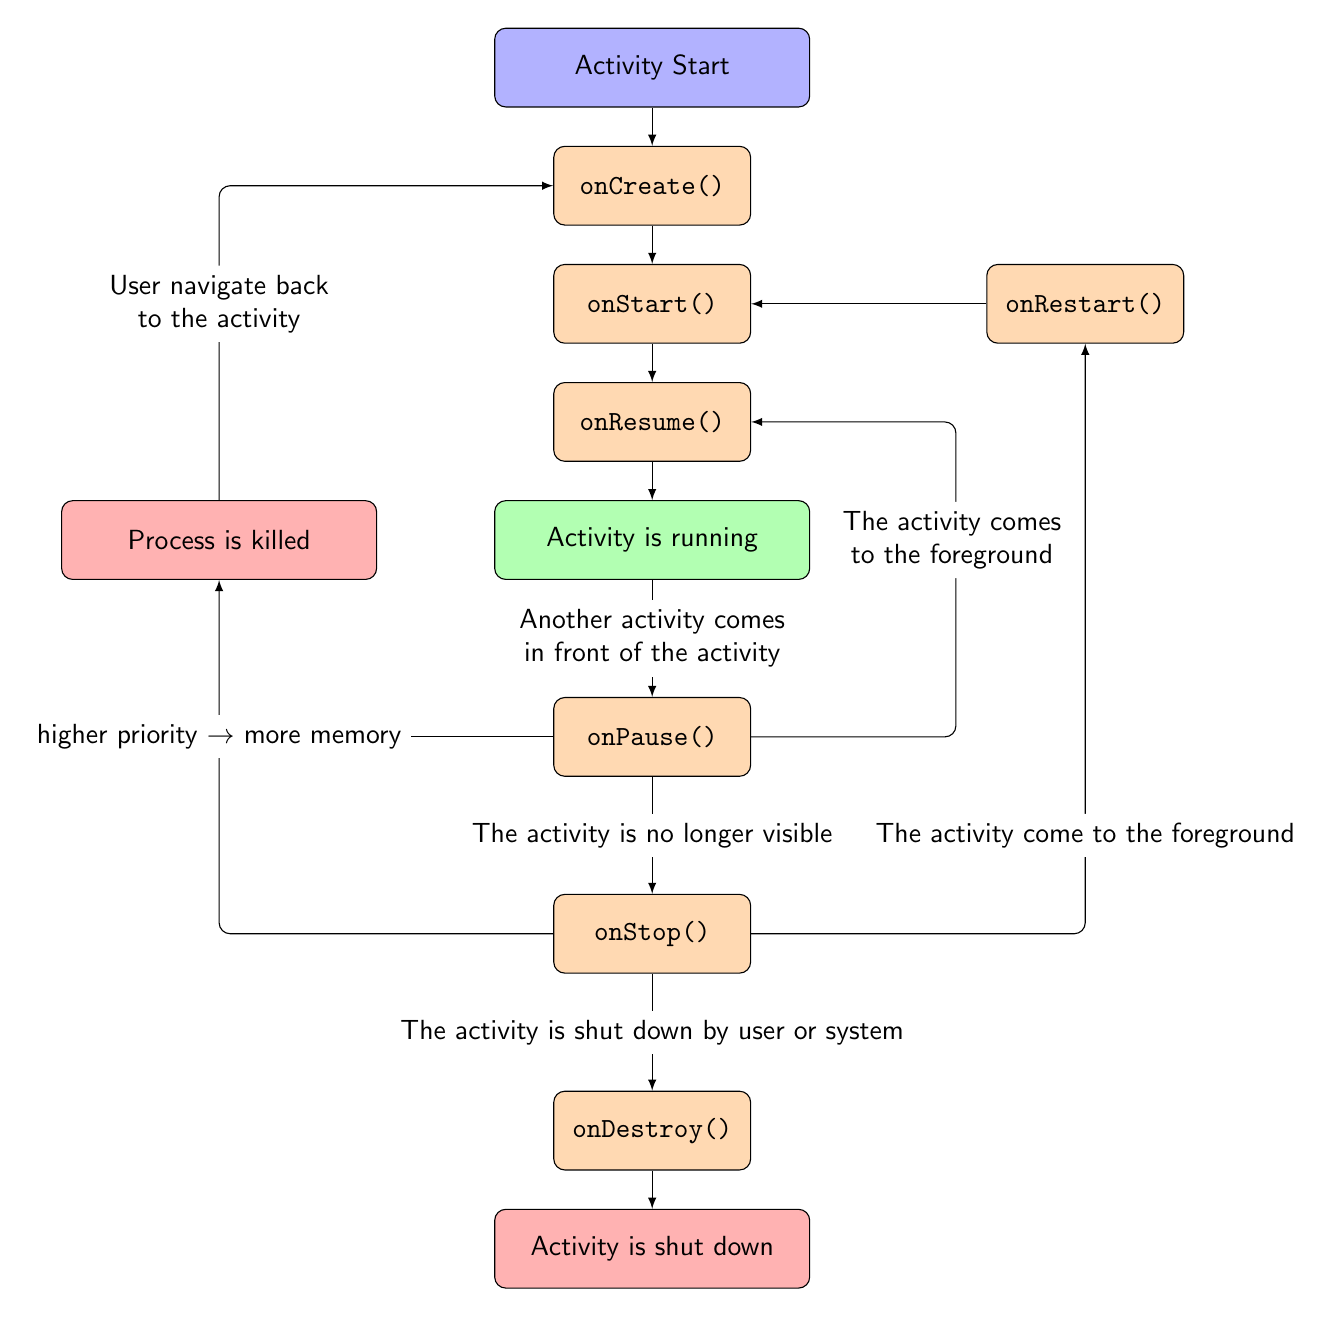
\begin{tikzpicture}[node distance=1.5cm, align=center]
        % place blocks of the flowchart
        \node[activityStart] (start) {Activity Start};
        \node[process] (onCreate) [below of=start] {onCreate()};
        \node[process] (onStart) [below of=onCreate] {onStart()};
        \node[process] (onRestart) [right of=onStart, xshift=4cm] {onRestart()};
        \node[process] (onResume) [below of=onStart] {onResume()};
        \node[activityRun] (activityRun) [below of=onResume] {Activity is running};
        \node[startStop] (processKilled) [left of=activityRun, xshift=-4cm] {Process is killed};
        \node[process] (onPause) [below of=activityRun, yshift=-1cm] {onPause()};
        \node[process] (onStop) [below of=onPause, yshift=-1cm] {onStop()};
        \node[process] (onDestroy) [below of=onStop, yshift=-1cm] {onDestroy()};
        \node[startStop] (activityShutdown) [below of=onDestroy] {Activity is shut down};
        % draw straight arrows and add nodes of text
        \path[->] (start) edge (onCreate)
                  (onCreate) edge (onStart)
                  (onStart) edge (onResume)
                  (onResume) edge (activityRun)
                  (activityRun) edge node[text width=6cm] {Another activity comes in front of the activity} (onPause)
                  (onPause) edge node[text width=6cm] {The activity is no longer visible} (onStop)
                  (onStop) edge node {The activity is shut down by user or system} (onDestroy)
                  (onDestroy) edge (activityShutdown);
        % draw right angle arrow and add nodes of text
        \draw[->, rounded corners] (onStop) -| node[yshift=1.25cm] {The activity come to the foreground} (onRestart);
        \draw[->] (onRestart) -- (onStart);
        \draw[->, rounded corners] (onStop) -| (processKilled);
        \node (onPause_left) at (onPause -| processKilled) {higher priority $\rightarrow$ more memory};
        \draw (onPause) -- (onPause_left);
        \draw[->, rounded corners] (onPause.east) -- ++(2.6, 0) -- ++(0, 2) -- ++(0, 2) -- node[text width=3cm, xshift=1.25cm, yshift=-1.5cm] {The activity comes to the foreground} (onResume.east);
        \draw[->, rounded corners] (processKilled) |- node[text width=4cm, yshift=-1.5cm] {User navigate back to the activity} (onCreate);
    \end{tikzpicture}
\end{document}